\documentclass[10pt]{article}
\usepackage[utf8]{inputenc}
\usepackage[T1]{fontenc}
\usepackage{amsmath}
\usepackage{amsfonts}
\usepackage{amssymb}
\usepackage[version=4]{mhchem}
\usepackage{stmaryrd}
\usepackage{graphicx}
\usepackage[export]{adjustbox}
\graphicspath{ {./images/} }

\begin{document}

    Stars can be well approximated as spherically symmetric objects, and hence the radial distance $r$ from the centre can be chosen as the only independent variable in modelling stellar interiors. The mass contained within a sphere of radius $r$ is denoted by $m(r)$. The luminosity $l(r)$ is defined as the net energy flowing outward through a spherical surface of radius $r$ per unit time. Other quantities of interest, for example, the density $\rho(r)$, temperature $T(r)$, hydrogen mass fraction $X(r)$, helium mass fraction $Y(r)$, and the nuclear energy generated per unit mass per unit time $\epsilon_{\text {nuc }}(r)$, are taken to be functions of $r$. Throughout this problem we shall neglect the effects of diffusion and gravitational settling of elements inside the star.

    The symbol "log" refers to logarithm to the base 10. The problem consists of three independent parts.
    
    \section*{(T11.1) Part 1: Inside a star}
    The graph below shows the variation of three structural quantities, $\mathrm{A}, \mathrm{B}$, and C , as functions of the fractional radius $r / R$ in a stellar model of mass $1 \mathrm{M}_{\odot}$ and age 4 GYr , where $R$ is the photospheric radius of the star. The values of the helium mass fraction at the (photospheric) surface, $Y_{\mathrm{s}}$, and the metallicity (mass fraction of all elements heavier than helium) at the (photospheric) surface, $Z_{\mathrm{s}}$, of the star are given by $\left(Y_{\mathrm{s}}, Z_{\mathrm{s}}\right)=(0.28,0.02)$. All quantities shown in the plots are normalised by their respective maximum values.\\
    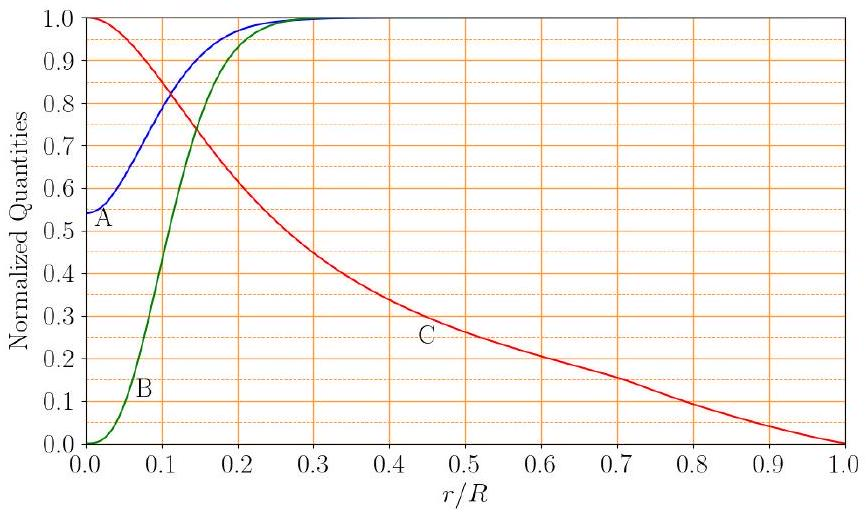
\includegraphics[max width=\textwidth, center]{2025_08_23_e94579452776a99c4850g-14(1)}\\
    (T11.1a) Identify the three quantities $\mathrm{A}, \mathrm{B}$, and C uniquely from among the five possibilities:
    
    $$
    T(r), l(r), \epsilon_{\mathrm{nuc}}(r), X(r), Y(r) .
    $$
    
    (Write $\mathrm{A} / \mathrm{B} / \mathrm{C}$ in the boxes beside the appropriate quantities in the Summary Answersheet. No justification is needed for your answer.)\\
    (T11.1b) What is the mass fraction of helium at the centre, $Y_{\mathrm{c}}$, of the star?\\
    (T11.1c) Sketch the remaining two quantities from the list of five (which were not identified as curves $\mathrm{A}, \mathrm{B}$, or C ) given in (T11.1a), as functions of $r / R$ on the same graph in the Summary Answersheet, and label by their respective quantities.
    
    \section*{(T11.2) Part 2: Evolving stars}
    Consider the evolution of a $1 \mathrm{M}_{\odot}$ star whose initial uniform composition is given by the mass fractions of helium, $Y_{0}=0.28$, and metals, $Z_{0}=0.02$. The figures below show the variation of different global quantities of this star as it evolves from ZAMS (Zero Age Main Sequence) till the end of helium burning in its core.
    
    The graph below shows the evolutionary track of the star on the HR diagram (plot of $\log L / L_{\odot}$ vs $\log T_{\text {eff }}$, where $L$ is the surface luminosity and $T_{\text {eff }}$ is the effective temperature).\\
    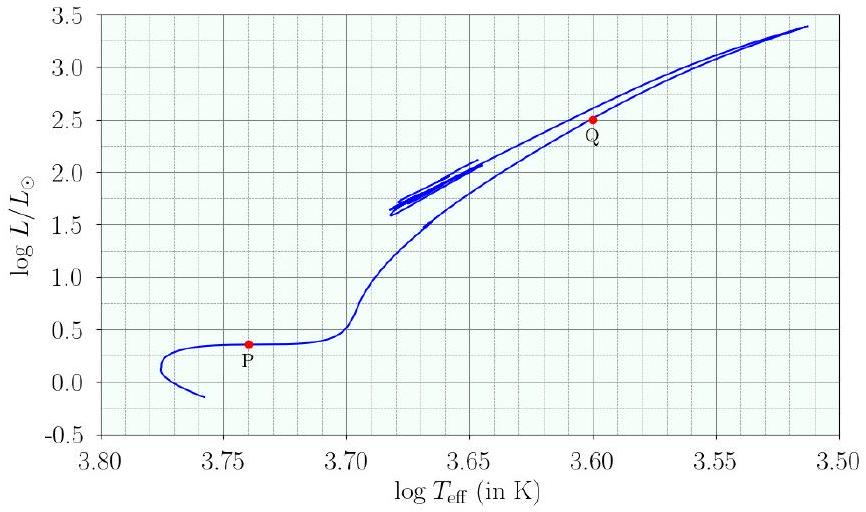
\includegraphics[max width=\textwidth, center]{2025_08_23_e94579452776a99c4850g-14}
    
    The figure below has four graphs which show the variation of $T_{\text {eff }}$ (in K), $L$ (plotted as $\log L / L_{\odot}$ ), $R$ (plotted as $\log R / R_{\odot}$ ), and $Y_{\mathrm{c}}$ with age (in $10^{9} \mathrm{yr}$ ) of the same star. In each of these four graphs, the insets show the variations of the respective quantities in detail between the ages of $11.86 \times 10^{9} \mathrm{yr}$ to $12.00 \times 10^{9} \mathrm{yr}$, for greater clarity.\\
    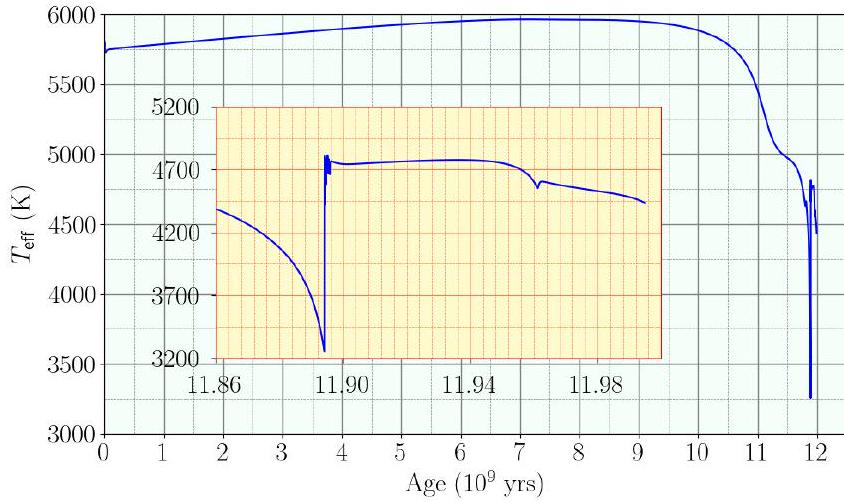
\includegraphics[max width=\textwidth, center]{2025_08_23_e94579452776a99c4850g-15(2)}\\
    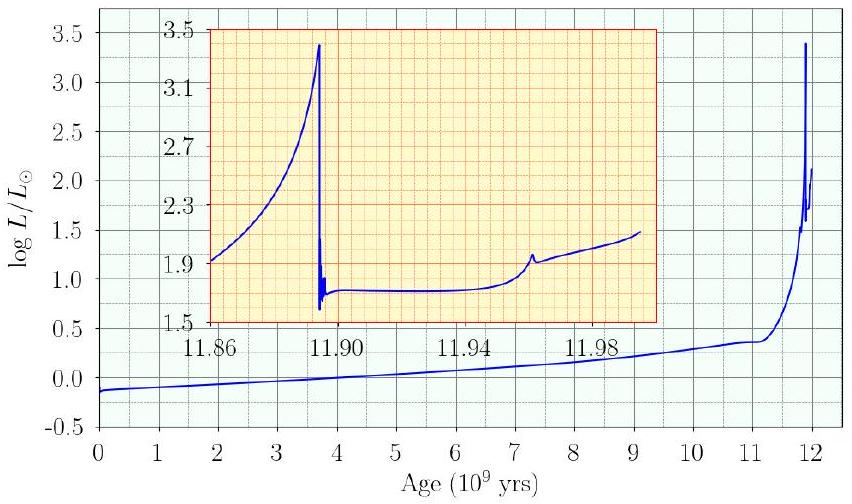
\includegraphics[max width=\textwidth, center]{2025_08_23_e94579452776a99c4850g-15(3)}\\
    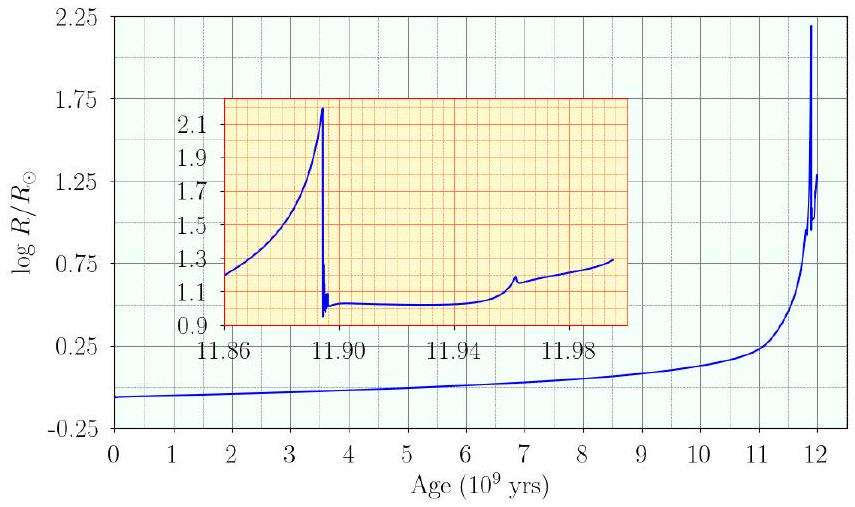
\includegraphics[max width=\textwidth, center]{2025_08_23_e94579452776a99c4850g-15}\\
    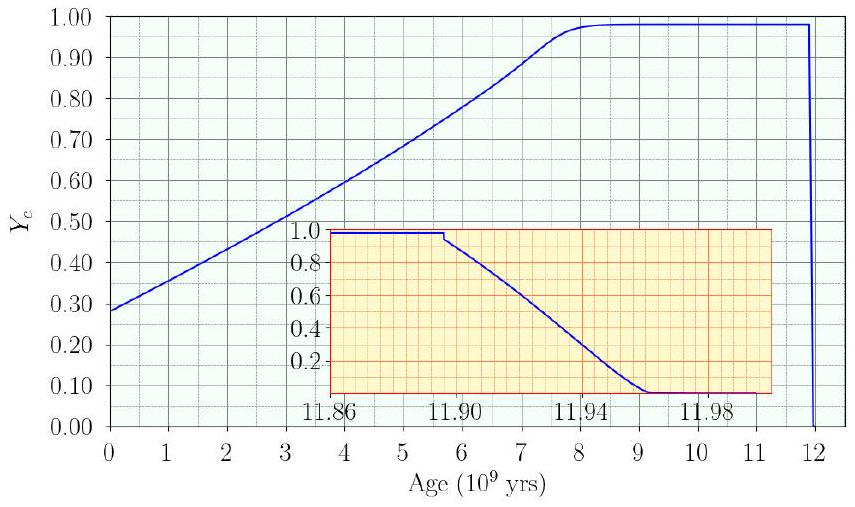
\includegraphics[max width=\textwidth, center]{2025_08_23_e94579452776a99c4850g-15(1)}
    
    Use these graphs to answer the questions below.\\
    (T11.2a) What is the approximate main sequence lifetime, $t_{\mathrm{MS}}$ (in years), of the star?\\
    (T11.2b) What is the approximate duration, $\Delta t_{\mathrm{He}}$ (in years), for which the star burns helium in its core?\\
    (T11.2c) What fraction, $f_{\mathrm{H}}$, of the initial amount of hydrogen at its centre has been burnt when the luminosity of the star is $1 \mathrm{~L}_{\odot}$ ?\\
    (T11.2d) What is the radius of the star, $R_{1}$ (in units of $R_{\odot}$ ) when $60 \%$ of the initial amount of hydrogen at its centre has been burnt?\\
    (T11.2e) What are the radii of the star, $R_{\mathrm{P}}$ and $R_{\mathrm{Q}}$ (in units of $\mathrm{R}_{\odot}$ ), corresponding to its positions P and Q , respectively, as marked on the HR-diagram?
    
    \section*{(T11.3) Part 3: Mass distribution inside a star}
    The equation that governs the distribution of mass inside a star is given by
    
    $$
    \frac{d m(r)}{d r}=4 \pi r^{2} \rho(r)
    $$
    
    It would be convenient to express this equation in terms of three dimensionless variables, namely, the fractional mass, $q$, the fractional radius, $x$, and the relative density, $\sigma$, that we define as
    
    $$
    q=m / M \quad x=r / R \quad \sigma=\rho / \bar{\rho}
    $$
    
    where $M$ and $R$ are the total mass and radius of the star, respectively, and $\bar{\rho} \equiv \frac{M}{\frac{4}{3} \pi R^{3}}$ is the average density of the star. For the particular star that we shall be considering in this part, the following information is given:
    
    \begin{itemize}
      \item The central density $\rho(x=0)=80 \bar{\rho}$
      \item Half of the star's mass is contained within the inner $25 \%$ of its total radius, and $70 \%$ of its mass is contained within the inner $35 \%$ of its total radius.
    \end{itemize}
    
    In all subsequent parts of this question, it will be sufficient to round off all derived numerical coefficients to within 0.005 .\\
    (T11.3a) Express the above equation describing the dependence of mass on radius in terms of $x$, $\frac{d q(x)}{d x}$ and $\sigma(x)$.
    
    To obtain the distribution of mass with radius, we need to know the density profile inside the star. For the purpose of this problem, we shall describe the variation of density with radius by approximate forms in two domains of $x$ :
    
    \begin{itemize}
      \item the inner part of the star: $0 \leq x \leq 0.32$
      \item the middle part of the star: $\overline{0.32}<x<0.80$
    \end{itemize}
    
    We do not make any approximation for the outermost part, i.e., $0.80 \leq x \leq 1.00$.
    
    \section*{Approximation for the middle part:}
    The variation of $\log \sigma$, as a function of $\log x$ in the middle part of the star is shown (by the black curve) in the graph below. We shall make a linear approximation (shown as a dashed red line in the graph) for $\log \sigma$ as a function of $\log x$ in the domain $-0.5<\log x<-0.1$, i.e., $0.32 \lesssim x \lesssim 0.80$ (shown by the green shaded domain). Further, we shall approximate the slope of this line by the nearest integer.\\
    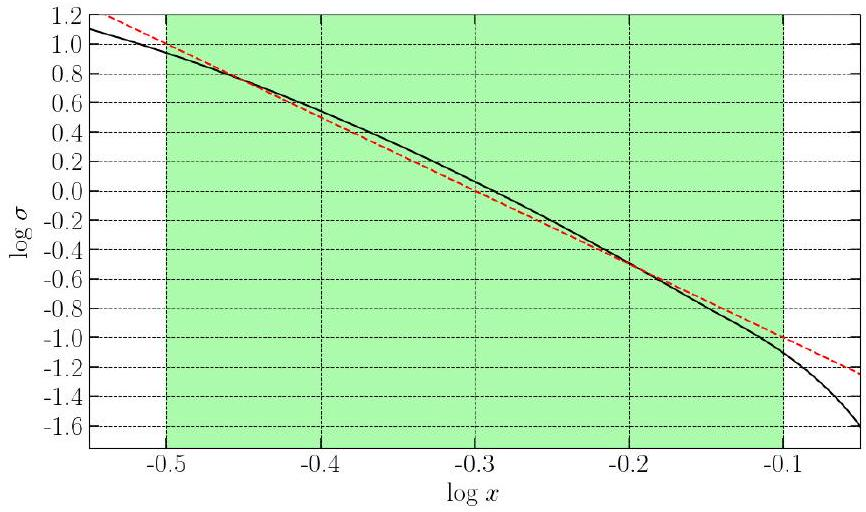
\includegraphics[max width=\textwidth, center]{2025_08_23_e94579452776a99c4850g-16}
    
    Use this approximation to write an expression for $\sigma(x)$ as a function of $x$ in the domain $0.32<x<0.80$.\\
    (T11.3c) Use the result of (T11.3b) to derive an expression for $q(x)$ in the domain $0.32<x<0.80$.
    
    \section*{(T11.3d) Approximation for the inner part:}
    In the inner part of the star ( $0 \leq x \leq 0.32$ ), the density may be approximated as a linear function of radius, i.e., $\sigma(x)=\bar{A} x+B$, where $A, B$ are constants. Determine $A$ and $B$, and hence obtain an expression for $q(x)$ in the domain $0 \leq x \leq 0.32$. Note that the approximations adopted in the previous part and this part may lead to small discontinuities in density or mass at $x=0.32$.\\
    (T11.3e) The expressions for $q(x)$ obtained in parts (T11.3c) and (T11.3d) are approximations that describe the variation of mass with radius quite well, but only in specific regions of the star. For the domain $0.80 \leq x \leq 1$ (for which we have not derived any expression), it is possible to use appropriate extrapolation from the neighbouring region. Use these approximate expressions and given data to sketch a smooth curve (without any discontinuities either in $q(x)$ or its derivative) for $q(x)$ vs $x$ for the entire star ( $0 \leq x \leq 1$ ) that represents the variation of mass with radius.

\end{document}